%%%%%%%%%%%%%%%%%%%%%%% CHAPTER - 4 %%%%%%%%%%%%%%%%%%%%\\
\chapter{Quantitative Analysis of the Morphological Complexity of Malayalam}
\label{Ch:MorphologicalComplexity} %%%%%%%%%%%%%%%%%%%%%%%%%%%%
\graphicspath{{Figures/chapter3-complexity/}}

\section{Introduction}

To lay the groundwork for the research works that aim to overcome the linguistic challenges in \gls{asr} for Malayalam, this chapter takes on the task of quantifying the morphological complexity of the language. To achieve this, we perform a quantitative analysis of the language's morphological complexity on a text corpus containing approximately 8 million words. The analysis utilises key parameters such as \gls{ttgr}, \gls{ttr}, and \gls{mattr} to determine the extent of the language's morphological complexity. We compare the obtained parameter values with those of other morphologically complex languages, gaining valuable insights into the unique linguistic characteristics of Malayalam.  The insights gained from this analysis will provide a better understanding of the linguistic characteristics of Malayalam, which will be useful in developing efficient and accurate \gls{asr} systems for the language. By establishing a comprehensive understanding of the morphological complexity of the Malayalam language, this chapter serves as a solid foundation for the subsequent research endeavours in the field of Malayalam \gls{asr}.

% This chapter presents a quantitative analysis on the morphological complexity
% of Malayalam language. Malayalam is a Dravidian language spoken in India,
% predominantly in the state of Kerala with about 38 million native speakers.
% Malayalam words undergo inflections, derivations and compounding leading to an
% infinitely extending lexicon.  %This paper also discusses the impact of morphological complexity on Automatic Speech Recognition task.

\section{Morphological Complexity}

Malayalam\footnote{\url{https://en.wikipedia.org/wiki/Malayalam}} is a language
with complex word morphology. Malayalam words undergo inflections, derivations
and compounding producing an infinite vocabulary \cite{thottingal2019finite}.
As a language with high morphological complexity it has a large number of
wordforms derived from a single root word (such as the English words
\textit{houses} and \textit{housing}, which stem from the same root word
\textit{house}). Morphological complexity can be measured either in terms of
the average number of grammatical features getting encoded into a word or in
terms of the diversity of word forms occurring in the text corpus of a
language. The former approach is called typological analysis and the latter one
is called corpus based analysis of morphological complexity
\cite{bentz2016comparison}. The level of morphological complexity present in a language can significantly impact applications such as \gls{asr}, where the accuracy of speech-to-text conversion largely depends on the underlying language model. Measuring this complexity is crucial in improving and adapting existing methods of \gls{nlp} to better suit the unique linguistic characteristics of the language \cite{gutierrez2018comparing}.


% This paper analyses the morphological complexity of Malayalam in terms of corpus based parameters namely, type-token growth rate (TTGR), type-token ratio (TTR) and moving average type-token ratio (MATTR). These parameters are formally defined in section \ref{methods}. The study is conducted on a Malayalam text corpus of 8 million words.

% \section{Literature Review}
% \label{sec:lr}

% \section{Problem Statement}
% \label{problem}

Malayalam has seven nominal case forms (nominative, accusative, dative,
sociative, locative, instrumental and genitive), two nominal number forms
(singular and plural) and three gender forms (masculine, feminine and neutral).
These forms are indicated as suffixes to the nouns. Verbs in Malayalam get
inflected based on tense (present, past and future), mood (imperative,
compulsive, promissive, optative, abilitative, purposive, permissive,
precative, irrealis, monitory, quotative, conditional and satisfactive), voice
(active and passive) and aspect (habitual, iterative, perfect)
\cite{nair2012grammar,thottingal2019finite}. The inflecting suffix forms vary
depending on the final phonemes of the root words. Words agglutinate to form
new words depending on the context \cite{asher1997malayalam}. Table
\ref{tab:morph-ml} gives examples of a few complex word formation in Malayalam.

\begin{table}[ht]

	\caption{Complex morphological word formation in Malayalam }
	\label{tab:morph-ml}

	\centering
	\begin{tabular}{p{4cm}p{3.5cm}p{4.7cm}}
		\hline \hline \bf Malayalam Word            & \bf English Translation  & \bf Remark                                                                                                           \\ \hline
		{\mal പെട്ടിയില്‍} ({\ipa  peʈʈijil})‍             & in the box                 & Nominal locative suffix to the word {\mal പെട്ടി‍} ({\ipa peʈʈi, box})‍                                                   \\

		{\mal കുട്ടിയോട്} ({\ipa kuʈʈijoːʈ})‍             & to the child               & Nominal sociative suffix
		to the word {\mal കുട്ടി} ({\ipa kuʈʈi, child})‍                                                                                                                                                    \\

		{\mal ആനക്കുട്ടി} ({\ipa aːnakkuʈʈi})‍           & baby elephant              & Compound word formed by agglutination of nouns {\mal ആന} ({\ipa aːna, elephant}) and {\mal കുട്ടി} ({\ipa kuʈʈi, baby}) \\

		{\mal ആനക്കുട്ടികളോട്‍} ({\ipa aːn̪akkuʈʈikaɭoːʈ})‍  & to the baby elephants      & Nominal sociative suffix to the plural form of the compound word {\mal ആനക്കുട്ടി} ({\ipa aːnakkuʈʈi, baby elephant})    \\

		{\mal ഉണര്‍ന്നിരിക്കണ്ട‍} ({\ipa uɳaɾn̪n̪iɾikkaɳʈa})‍  & do not stay awake          & Negative imperative mood of the verb {\mal ഉണരുക} ({\ipa uɳaɾuka, be awake})                                          \\

		{\mal പാടിക്കൊണ്ടിരിക്കും} ({\ipa paːʈikkoɳʈiɾikkum})‍ & will be singing            & Future tense iterative aspect of the verb {\mal പാടുക} ({\ipa paːʈuka, to sing})                                       \\

		\hline
	\end{tabular}

\end{table}

The productive word formation and morphological complexity of Malayalam are
documented qualitatively in the domain of grammatical studies. However a
quantitative study on the same is not yet available for Malayalam language.
Adoption of general \gls{nlp} solutions of high resource languages like English is
not feasible in the setting of morphologically complex languages. A functional
morphology analyser, Mlmorph addresses the morphological complexity of
Malayalam applying grammatical rules over root word lexicon
\cite{thottingal2019finite}. Quantification of linguistic complexity is
important to adapt and improve various \gls{nlp} applications like automatic speech
recognition, parts of speech tagging and spell checking
\cite{georgiev-etal-2012-feature,kipyatkova2014study,pakoci_using_2019,pirinen2014weighted}. This study aims at quantifying the morphological complexity of Malayalam in
terms of corpus linguistic parameters.

\section{Dataset}

This study is performed on Malayalam running text from Wikipedia articles. The
Malayalam Wikipedia dump is curated and published by Swathanthra Malayalam
Computing (SMC) as SMC Corpus \cite{smctext}. It consists of 62302
articles. The Malayalam running text often has foreign words, punctuation and
numerals present in it. The corpus is first cleaned up to eliminate non
Malayalam content and punctuation. It is then Unicode normalised
\cite{davis2001unicode}. The cleaned up corpus contained 8.14 million Malayalam
words. The nature of the text is formal encyclopedic Malayalam.

\section{Experimental Details}

An element of the set of distinct wordforms in a running text is called a  type. Every instance of a type in the running text is called a  token.
For example, in the sentence, {\em To be or not to be is the question}, there
are 7 types and 9 tokens. The types {\em to} and {\em be} repeat two times
each. The relationship between the count of types and tokens is an indicator of
vocabulary richness, morphological complexity and information flow
\cite{gutierrez2018comparing}. The \gls{ttr} is a simple baseline
measure of morphological complexity \cite{kettunen2014can}. \gls{ttr} is calculated
by the formula defined in equation \ref{eq:TTR}, where \gls{typecount} is the count of types
and \gls{tokencount} is the count of tokens.
\begin{equation}
	TTR = \frac{V}{N}
	\label{eq:TTR}
\end{equation}

The type count gets expanded due to productive morphology and higher values of
TTR correspond to higher morphological complexity \cite{bentz2016comparison}.
However TTR is affected by the token count, $N$ \cite{covington2010cutting}.
Larger the corpus, it is more likely that the new tokens belong to the types
that have occurred already. The value of TTR gets smaller with the increase in
token count. Computing TTR over incrementally larger corpus can indicate how
the TTR varies with the token count. In this study, TTR is computed with
different token counts starting with 1000 and increasing up to the entire corpus
size. This has enabled comparison of Malayalam with the morphological
complexity of other languages whose TTR values are available in literature for
different token counts.

The \gls{ttgr} curve is obtained by plotting the graph of
token count vs. type count. It indicates how many new types appear with the
increase in the token count. If the slope of the growth rate curve reduces and
approaches a horizontal line, at a lower value of token count, it indicates a
simple morphology \cite{bharadwaja2007statistical}. For a morphologically
complex language, the type count continues to grow with the token count
\cite{htay2007statistical}.

The \gls{mattr} computes the relationship between
types and tokens that is independent of the text length. Its efficient
implementation by Covington et al. has been used by Kettunen to compare the
morphological complexity of different European languages
\cite{covington2010cutting,kettunen2014can}. The algorithm to compute MATTR is
as described in Algorithm \ref{alg:mattr} \cite{fidler2018taming}:

% \begin{algorithm}[ht]
% 	\KwData{}
% 	\KwResult{MATTR}
% 	N $\gets$ length of corpus\;
% 	L $\gets$ length of window (L<N)\;
% 	start $\gets$ initial position of window \;
% 	i = start $\gets$ index of window position\;

% 	\While{$i \le (N-L+1)$}{
% 		$V_i = type\ count\ in\ the\ window\ [i, i+L-1]$\;
% 		$TTR(i) = \frac{V_i}{L}$\;
% 		$i = i+1$\;
% 	}
% $	MATTR(L) = \frac{\sum_{i=1}^{N-L+1} TTR(i)}{N-L+1} $

% 	\caption{Computation of MATTR}
% \end{algorithm}

% \begin{algorithm}
% 	\caption{Computation of MATTR}\label{mattr-algorithm}
% 	\begin{algorithmic}[1]
% 	\Require{A text Corpus, C}
% 	\Procedure{MATTR}{C}
% 	    \State{N $\gets$ length of corpus} 
%         \State{L $\gets$ length of window (L<N)}
%         \State {start $\gets$ initial position of window}
%          \State {i = start } \Comment{index of window position}
% 	    \While{$i \le (N-L+1)$} 
%             \State{$V_i = type\ count\ in\ the\ window\ [i, i+L-1]$}
%     	    \State{$TTR(i) = \frac{V_i}{L}$}
%     	    \State{$i = i+1$}
%     	\EndWhile
%     \State{$MATTR(L) = \frac{\sum_{i=1}^{N-L+1} TTR(i)}{N-L+1} $}
% 	\EndProcedure{}
% 	\end{algorithmic}
% \end{algorithm}

\begin{algorithm}[ht]
	\caption{Computation of MATTR}\label{mattr-algorithm}
    \label{alg:mattr}
	\begin{algorithmic}[1]
		\Require{A text Corpus, C}
		% \Return{MATTR}
		\Procedure{MATTR}{}
		\State{N $\gets$ length of corpus}
		\State{L $\gets$ length of window (L<N)}
		\State {start $\gets$ initial position of window}
		\State {i = start } \Comment{index of window position}
		\While{$i \le (N-L+1)$}
		\State{$V_i = type\ count\ in\ the\ window\ [i, i+L-1]$}
		\State{$TTR(i) = \frac{V_i}{L}$}
		\State{$i = i+1$}
		\EndWhile
		\State{$MATTR(L) = \frac{\sum_{i=1}^{N-L+1} TTR(i)}{N-L+1} $}
		\EndProcedure
	\end{algorithmic}
\end{algorithm}

The corpus with $N$ tokens is divided into the overlapped subtexts of the same
length, say \gls{windowlength}, the window length. Window moves forward one token at a time
and TTR is computed for every window. MATTR is defined as the mean of the
entire set of TTRs \cite{covington2010cutting}. In this work, $L$ is chosen as
500, enabling comparison with other languages in the study by Kettunen, where
the window length is 500 \cite{kettunen2014can}. %With a smoothly moving window, TTR value is obtained for every window positions in the text except for those less than one window length from the beginning \cite{covington2010cutting}. 

\section{Result and Discussion}
\begin{figure}[ht]
	\begin{center}

		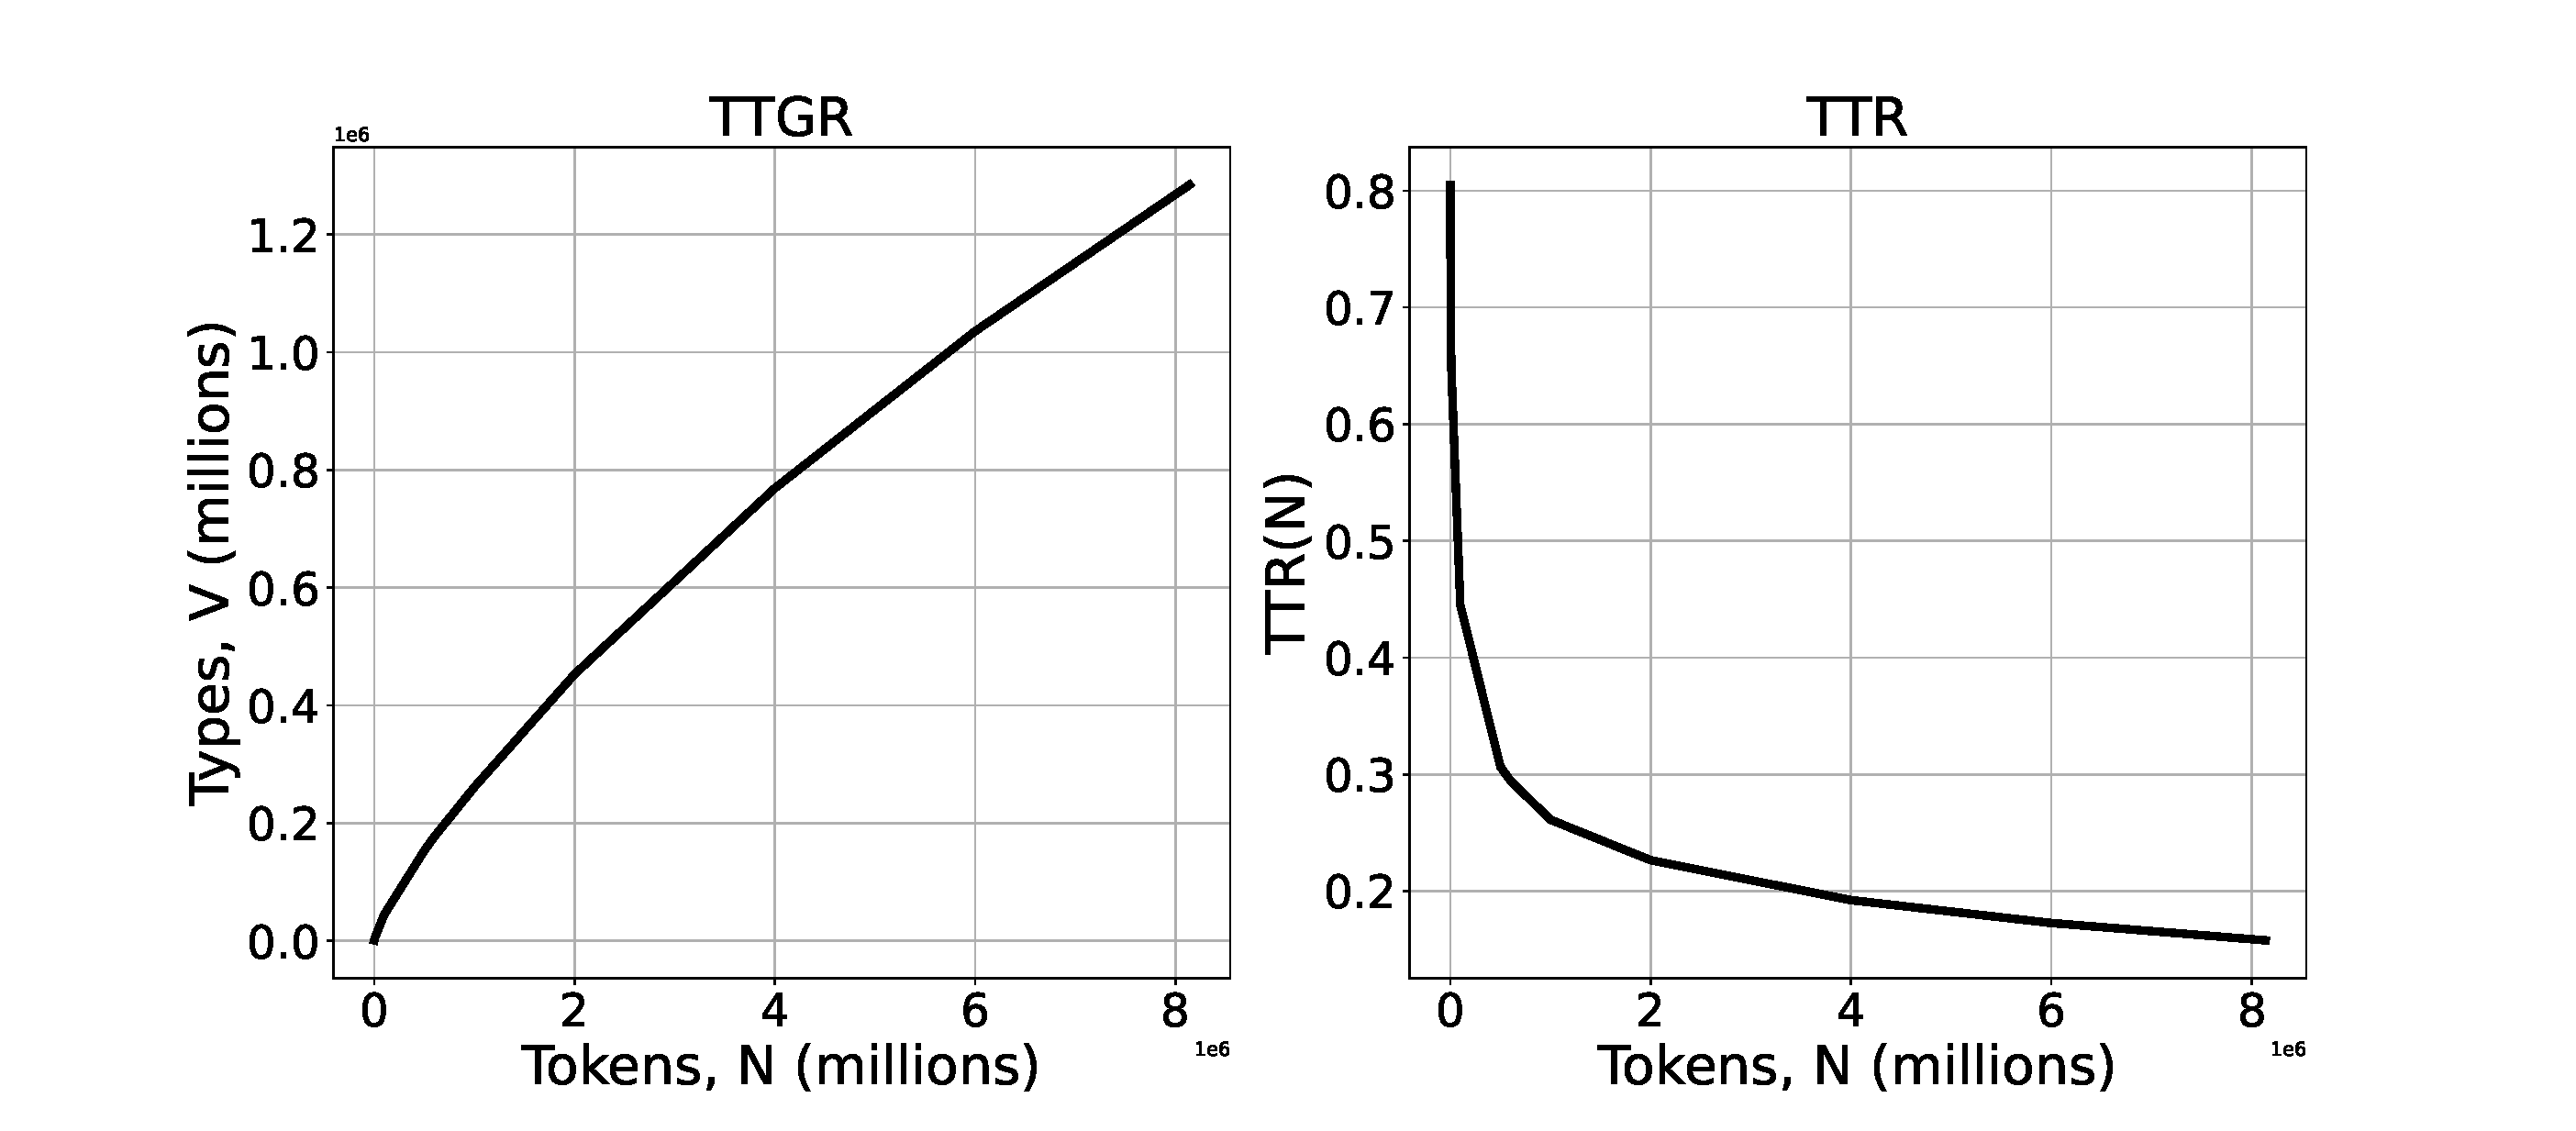
\includegraphics[width=\textwidth]{tsd1030a.eps}
		\caption{TTGR and TTR plot of Malayalam for SMC Corpus of Wikipedia text}
		\label{fig:TTR_N}

	\end{center}
\end{figure}


Counting the types and tokens on SMC Corpus \cite{smctext}, TTGR and TTR curves are
plotted. Fig. \ref{fig:TTR_N} shows the TTGR curve on the left and the TTR on the
right. TTGR curve shows a steep rise initially. As the token count reaches 8
million, the type count is around 1.2 million. But the curve does not flatten
even at that token count. This pattern is a common property of Dravidian
languages as many unseen wordforms appear as the corpus size is increased
\cite{bharadwaja2007statistical}. TTR is very high at around 0.82 when the
token count is 1000. TTR reduces to around 0.44 when the token count is 0.1
million and finally flattens to a value of 0.16 for the full corpus of 8
million tokens.

\begin{figure}[ht]
	\begin{subfigure}{.5\textwidth}
		\centering
		\includegraphics[width=\linewidth, height=5cm]{tsd1030b.eps}
		\caption{}
		\label{fig:TTR_comparison1}
	\end{subfigure}
	\begin{subfigure}{.5\textwidth}
		\centering
		\includegraphics[width=\linewidth, height=5cm]{tsd1030c.eps}
		\caption{}
		\label{fig:TTR_comparison2}
	\end{subfigure}
	\caption{Comparison of Malayalam TTR with that of European Union Constitution Corpus  and DoE-CIIL Corpus}
	\label{fig:TTR_comparison}
\end{figure}

To compare the TTR obtained for Malayalam with that of other languages, we have
used the results reported for European languages by Kettunen and for Indian
languages by Kumar et al. \cite{kettunen2014can,bharadwaja2007statistical}.
Fig.s \ref{fig:TTR_comparison1} and \ref{fig:TTR_comparison2} illustrates the
comparison. Only those languages with the highest reported TTRs in the
respective works and English are used for comparison. The token size (in
millions) used for computing TTRs  is indicated for each
language. Malayalam clearly shows more morphological complexity than the
European languages, Finnish, Estonian, Czech, Slovak, English and Spanish in
terms of TTR values. TTR values for Malayalam when compared with
other Indian languages Marathi, Hindi, Tamil, Kannada and Telugu clearly indicates a
higher level of morphological complexity for Malayalam.



\begin{figure}[htpb]
	\begin{center}

		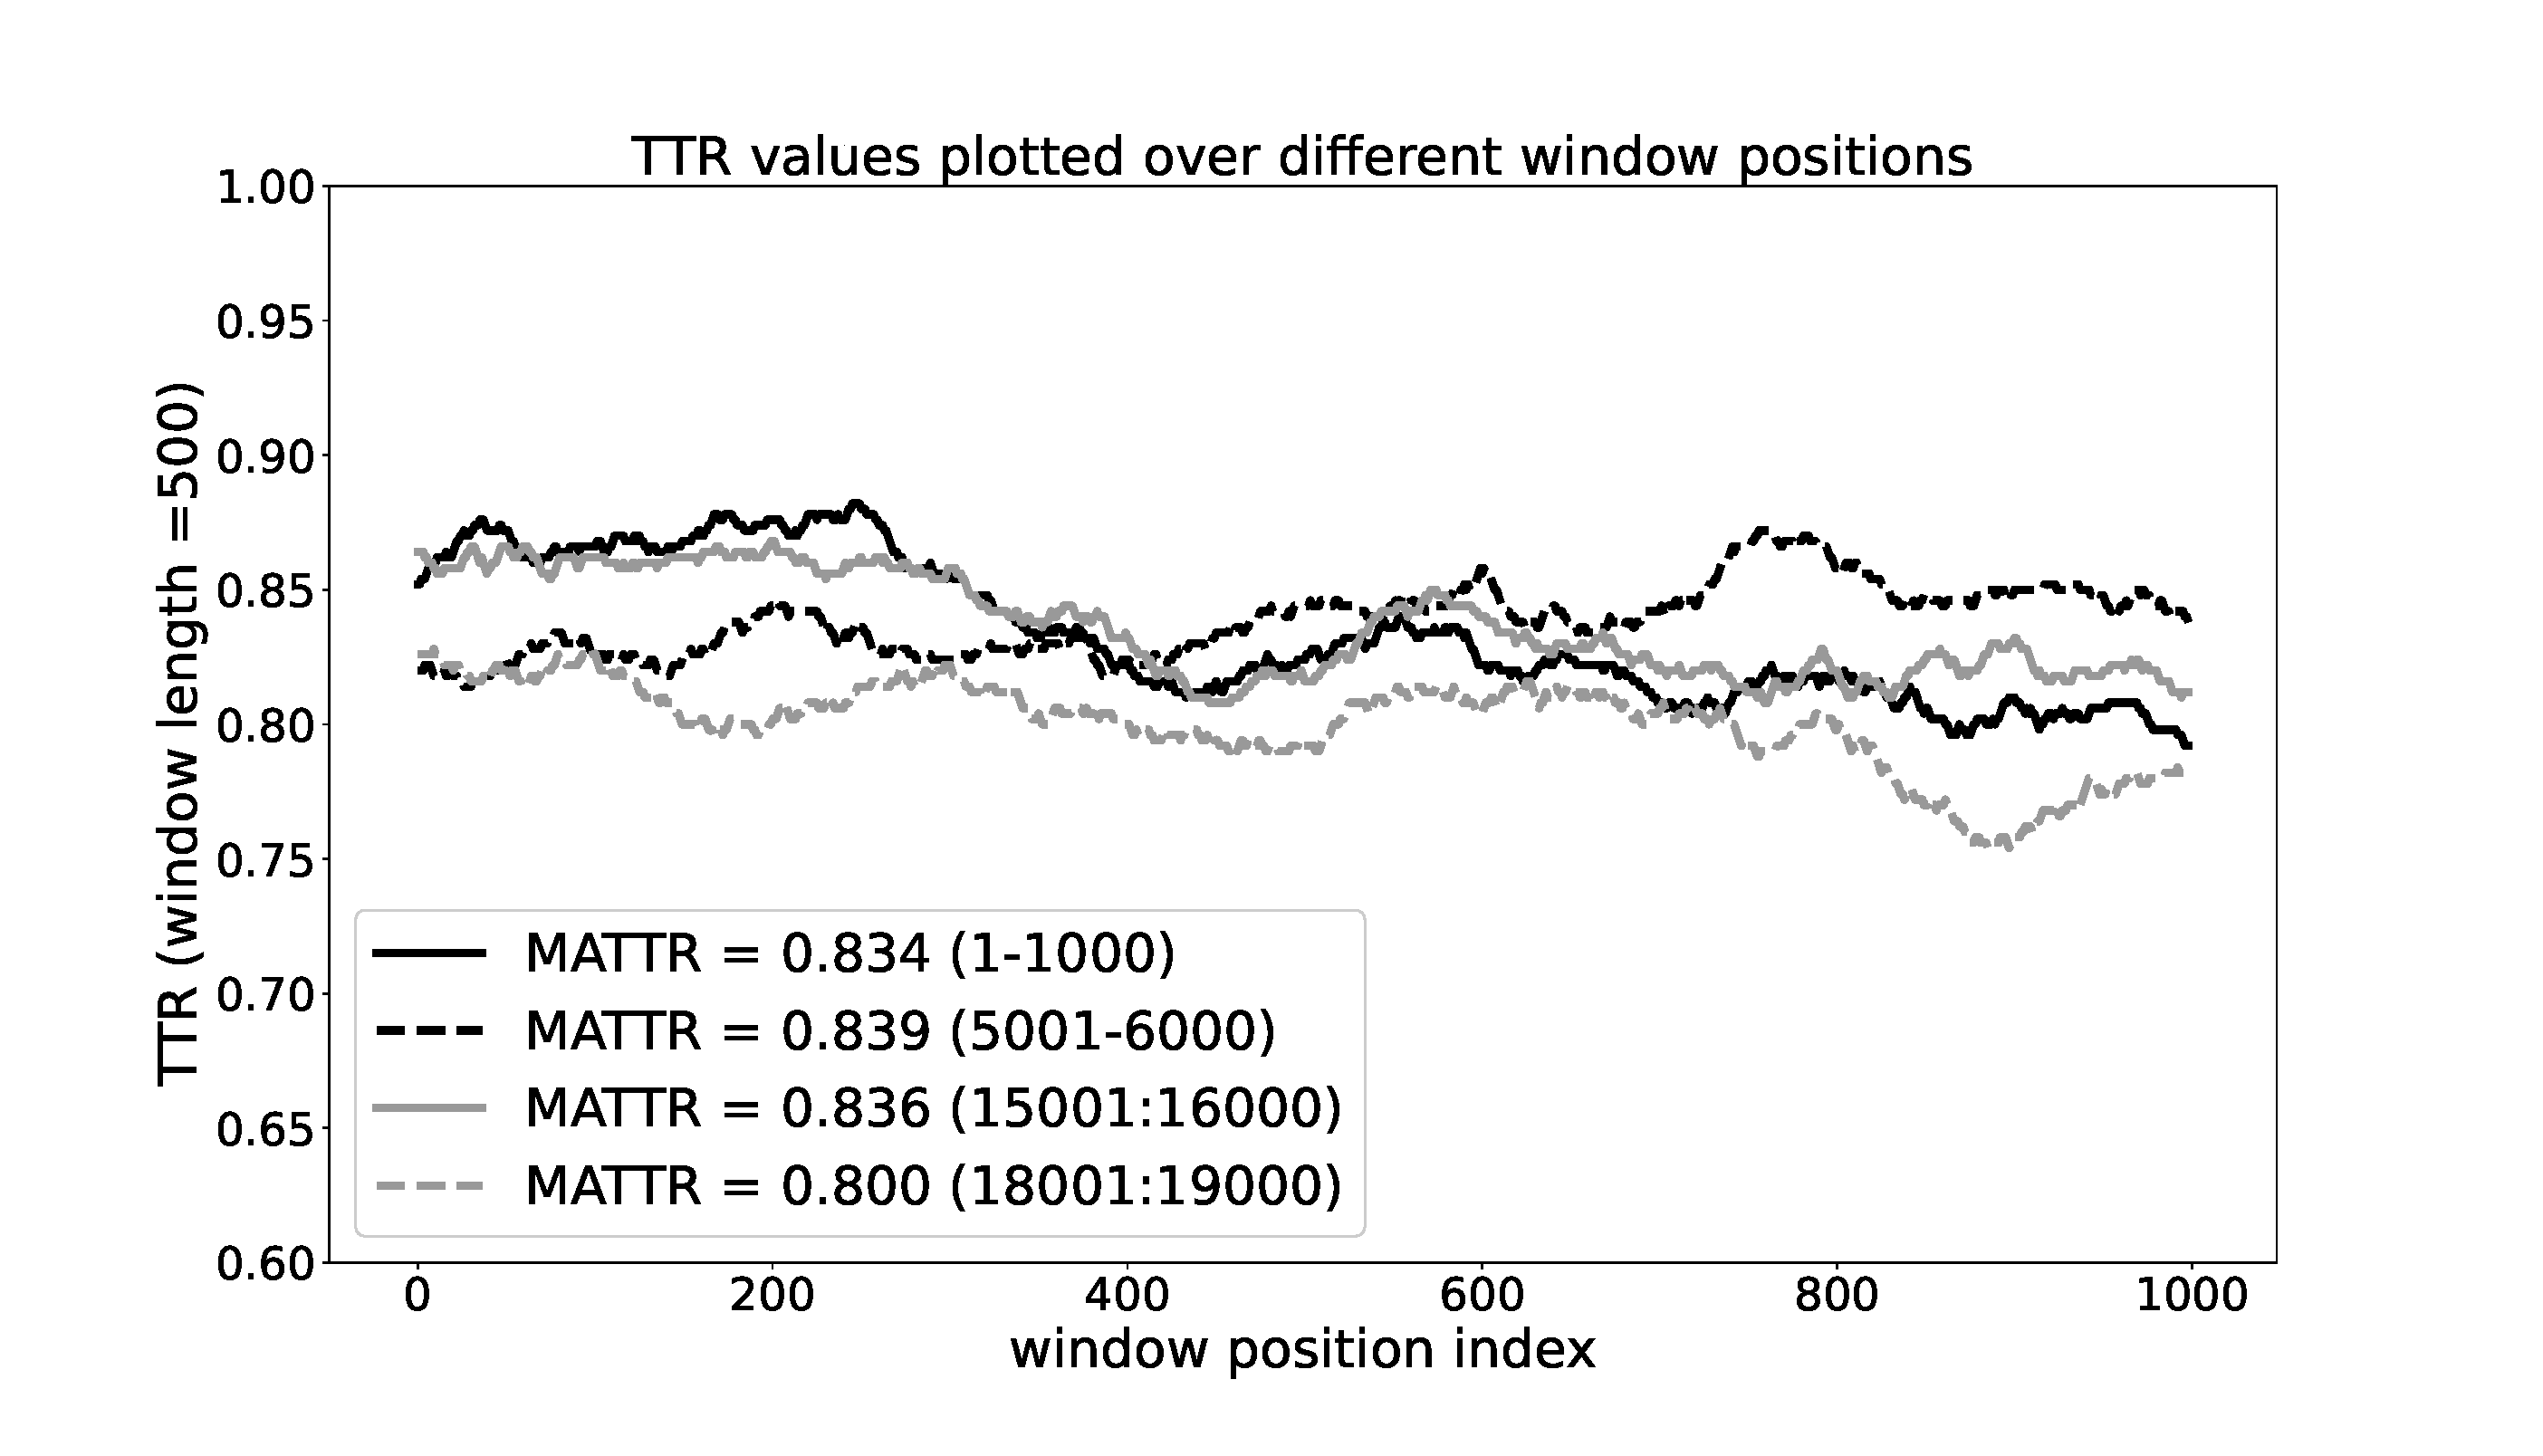
\includegraphics[width=0.8\textwidth]{tsd1030d.eps}
		\caption{TTR plotted at different segments of the SMC corpus for 1000 window positions}
		\label{fig:MATTRfig}

	\end{center}
\end{figure}

MATTR is computed with window length, $L=500$ over different segments of the
SMC corpus. TTR values for the segments with window position index
1-1000, 5001-6000, 15001-16000 and 18001-19000 are shown in Fig.
\ref{fig:MATTRfig}. These segments gave MATTR values 0.834, 0.839, 0.836 and 0.800
respectively. Computing MATTR with 0.1 million tokens of SMC corpus
resulted in a value 0.806 for Malayalam. Kettunen has reported MATTR values on
 European Union constitution corpus with each language having a token
count slightly above 0.1 million \cite{kettunen2014can}. The MATTR values reported by Kettunen with the values obtained for Malayalam is
plotted in Fig. \ref{fig:MATTRcomp}. It clearly indicates a higher degree of
morphological complexity for Malayalam in terms of MATTR on a formal text
corpus. An equivalent comparison with other Indian languages could not be done
due to non availability of reported studies.

\begin{figure}[ht]
	\begin{center}

		\includegraphics[width=0.95\textwidth]{tsd1030e.eps}
		\caption{Comparison of MATTR values computed for Malayalam on SMC Corpus with that of European Union Constitution Corpus}
		\label{fig:MATTRcomp}
		% 
	\end{center}
\end{figure}

\section{Summary}

To conclude, this chapter provides a quantitative analysis of the morphological complexity of Malayalam language on a formal text corpus of approximately 8 million words. The analysis has revealed a high degree of morphological complexity in Malayalam, as evidenced by the values of TTR and MATTR. It is essential to consider this aspect of the language's complexity while developing natural language processing applications, such as \gls{asr}, spell-checking, and part-of-speech tagging, for Malayalam. To accomplish this, we must create subword-based \gls{lm}s and \gls{pl}s for \gls{asr}, and perform a morphological analysis of words for POS tagging and spelling correction. By taking these crucial steps, we can develop more efficient and accurate \gls{nlp} tools that cater to the unique linguistic characteristics of Malayalam.